%% SFDCT — IEEE conference paper. Compile on Overleaf (no local TeX in dev env).
%% latexmk -pdf main.tex   (needs IEEEtran.cls + graphicx + booktabs + amsmath)
\documentclass[conference]{IEEEtran}
\IEEEoverridecommandlockouts
\usepackage{cite}
\usepackage{amsmath,amssymb,amsfonts}
\usepackage{graphicx}
\usepackage{booktabs}
\usepackage{xcolor}
\usepackage[hidelinks]{hyperref}
\graphicspath{{figures/}}
\newcommand{\todo}[1]{\textcolor{red}{[TODO: #1]}}

\begin{document}

\title{SFDCT: A Floor-Preserving Spatial--Frequency Fusion for\\
Cross-Dataset Deepfake Detection under eKYC Operating Points}

\author{\IEEEauthorblockN{Le Ngoc Thanh}
\IEEEauthorblockA{Faculty of Information Technology\\
The University of Danang -- University of Science and Technology\\
Da Nang, Vietnam}}

\maketitle

\begin{abstract}
Deepfake face forgery threatens electronic Know-Your-Customer (eKYC) pipelines in
banking, where detectors trained on one corpus often degrade sharply on unseen
manipulations. We present \textbf{SFDCT}, a hybrid spatial--frequency detector that augments an
EfficientNet-B4 backbone with a block-wise $8{\times}8$ DCT branch and fuses the two streams
through a \emph{zero-initialized} gated cross-attention. The zero-init gate makes the model at
initialization \emph{mathematically identical} to the calibrated backbone, giving a
\emph{floor-preserving} guarantee (never worse than B4 at init) that is directly valuable for
eKYC, where the operating threshold is calibrated on the baseline and must not regress.
We deliberately \textbf{do not claim state-of-the-art AUC}: under the standardized
DeepfakeBench cross-dataset protocol (train FaceForensics++ c23, test Celeb-DF-v2), SFDCT
reaches \textbf{0.7572} frame-AUC versus \textbf{0.7497} for B4 ($\Delta{=}{+}0.0075$), a gain that a
bootstrap confidence interval shows lies \emph{within noise}. Our contributions are therefore framed
honestly as (i) a floor-preserving fusion mechanism, (ii) a regulation-aware eKYC operating-point
evaluation that decomposes errors via the ISO/IEC~30107-3 taxonomy, and (iii) a small Vietnamese-face
deepfake \emph{test-only} resource. We report all numbers from a single seed and openly discuss the
limitations.
\end{abstract}

\begin{IEEEkeywords}
deepfake detection, eKYC, block-wise DCT, spatial--frequency fusion, cross-dataset generalization
\end{IEEEkeywords}

\section{Introduction}
Electronic Know-Your-Customer (eKYC) lets customers open accounts and authorize transactions
remotely from a selfie. This convenience opens an attack surface: low-cost \emph{deepfakes} can
synthesize a convincing face and bypass biometric verification, enabling identity fraud. In Vietnam,
Circular 17/2024/TT-NHNN mandates biometric authentication for certain banking transactions. We note
explicitly that \textbf{this circular states a \emph{qualitative} requirement and does not prescribe a
numeric error threshold}; to make the requirement measurable we \emph{adopt} an operating point of
$\text{FPR}\le 5\%$ following the ISO/IEC~30107-3 convention (BPCER20)~\cite{iso30107,tt17_2024}.

A central obstacle is the \emph{in-dataset-high / cross-dataset-low} paradox: a detector with near-perfect
in-domain accuracy can collapse on a new corpus~\cite{yan2023deepfakebench}. The core hypothesis we
build on is that up-sampling/GAN artifacts are weak in the spatial domain but more visible in
mid/high 2D-DCT frequency bands, so spatial and frequency cues should be \emph{complementary}.

\textbf{We do not claim a new mechanism or SOTA AUC.} Instead, this paper makes three contributions:
\begin{itemize}
  \item \textbf{C1 (architecture/safety).} A \emph{floor-preserving} spatial--frequency fusion:
  a block-DCT branch fused into B4 by a zero-initialized gated cross-attention, so the model at
  initialization equals the calibrated backbone (Sec.~\ref{sec:method}).
  \item \textbf{C2 (evaluation).} A regulation-aware eKYC operating-point evaluation that calibrates
  the decision threshold at $\text{FPR}\le 5\%$ and decomposes errors with the ISO/IEC~30107-3
  taxonomy on forgery (Sec.~\ref{sec:ekyc}).
  \item \textbf{C3 (resource).} A small \emph{test-only} Vietnamese-face deepfake set for the eKYC
  operating point (\todo{collect; described in Sec.~\ref{sec:limits}}).
\end{itemize}
Two methodological pillars support these: a DeepfakeBench-faithful ablation protocol and honest
bootstrap-CI reporting that lets us \emph{refute our own} AUC gain when it is within noise.

\section{Related Work}
\textbf{Frequency-domain forgery detection.} F3-Net mines learnable frequency bands and local
statistics~\cite{qian2020f3net}; SPSL uses the phase spectrum~\cite{liu2021spsl}; high-frequency
SRM residuals improve generalization~\cite{luo2021srm}; FcaNet generalizes channel attention with
multi-spectral 2D-DCT~\cite{qin2021fcanet}; FDFL adds a single-center loss~\cite{li2021fdfl};
FreqDebias mixes amplitude spectra to fight spectral bias~\cite{freqdebias2025}. SFDCT does not
introduce a new frequency operator; it \emph{unifies} five such levers (S1--S5) inside a single
block-DCT domain. On the standardized DeepfakeBench scale, SPSL (0.7650) and SRM (0.7552) remain
at or above our naive SFDCT (0.7572): \textbf{we do not outperform SPSL.}

\textbf{Spatial--frequency fusion and zero-init gating.} Most two-stream detectors fuse by
concatenation or plain cross-attention without any guarantee against regression. Residual zero-init
(ReZero~\cite{bachlechner2021rezero}) and zero-gated cross-attention (Flamingo~\cite{alayrac2022flamingo})
are known in other domains. The closest work is SFCL-HCMF~\cite{sfclhcmf2025}, which also pairs a
block-DCT $8{\times}8$ YCbCr branch with EfficientNet-B4 and gated cross-modal fusion; the decisive
difference is its gate $\sigma(\gamma)$ initializes at $0.5$ (no floor), whereas our $\alpha{=}0$ yields a
mathematical floor $\ge$ B4. SFDCT's C1 is thus a \emph{new application/combination}, not a new mechanism.

\textbf{Cross-dataset / eKYC evaluation.} TPR@FPR for deepfakes and APCER/BPCER/ACER from PAD
(ISO/IEC~30107-3~\cite{iso30107}) already exist; ethnicity-specific deepfake sets (e.g.\ KoDF) are
common. Our delta is narrow and honest: anchoring the operating point to the Vietnamese eKYC context
and providing a VN-face test instance.

\section{Method}\label{sec:method}
\textbf{Spatial branch.} EfficientNet-B4~\cite{tan2019efficientnet} pretrained on ImageNet produces a
feature map $x$ from a $256{\times}256$ aligned face crop.

\textbf{Frequency branch.} The crop is converted to YCbCr; a block-wise $8{\times}8$ 2D-DCT is applied,
its log-magnitude is taken and grouped into 16 zigzag bands (with an option to drop the DC and lowest
bands to curb content leakage). This yields a frequency feature $f$.

\textbf{Floor-preserving fusion.} The two streams are merged by a gated cross-attention
\begin{equation}
\text{feature} = x + \alpha \cdot \mathrm{CrossAttn}(x, f), \qquad \alpha\!\leftarrow\!0 \text{ at init},
\end{equation}
where $\alpha$ is a learnable scalar gate initialized to $0$. At initialization the model is identical
to B4, guaranteeing performance never below the calibrated backbone; a positive learned $\alpha$ is
direct evidence the frequency branch is used (Fig.~\ref{fig:gate}).

\textbf{Five frequency levers (S1--S5).} Adapted into the single block-DCT domain: S1 DCT coefficient
sign (cf.\ SPSL), S2 DCT on SRM residual (cf.\ SRM), S3 DCT-FoMixup + dual consistency (cf.\ FreqDebias),
S4 multi-spectral DCT attention (cf.\ FcaNet), S5 single-center loss (cf.\ FDFL). All are off in
``naive SFDCT''.

\textbf{Training.} Adam ($\text{lr}{=}2\!\times\!10^{-4}$, weight decay $5\!\times\!10^{-4}$), batch 32,
32 frames/video, $256{\times}256$, 10 epochs, seed 1024, cross-entropy; checkpoint by best test-AUC.

\section{Experiments}\label{sec:exp}
\textbf{Protocol.} We follow DeepfakeBench~\cite{yan2023deepfakebench}: train on FaceForensics++
c23~\cite{rossler2019faceforensics}, test cross-dataset on Celeb-DF-v2~\cite{li2020celebdf}; the headline
metric is frame-level AUC. Fig.~\ref{fig:dist} shows the class distributions.

\begin{figure}[t]\centering
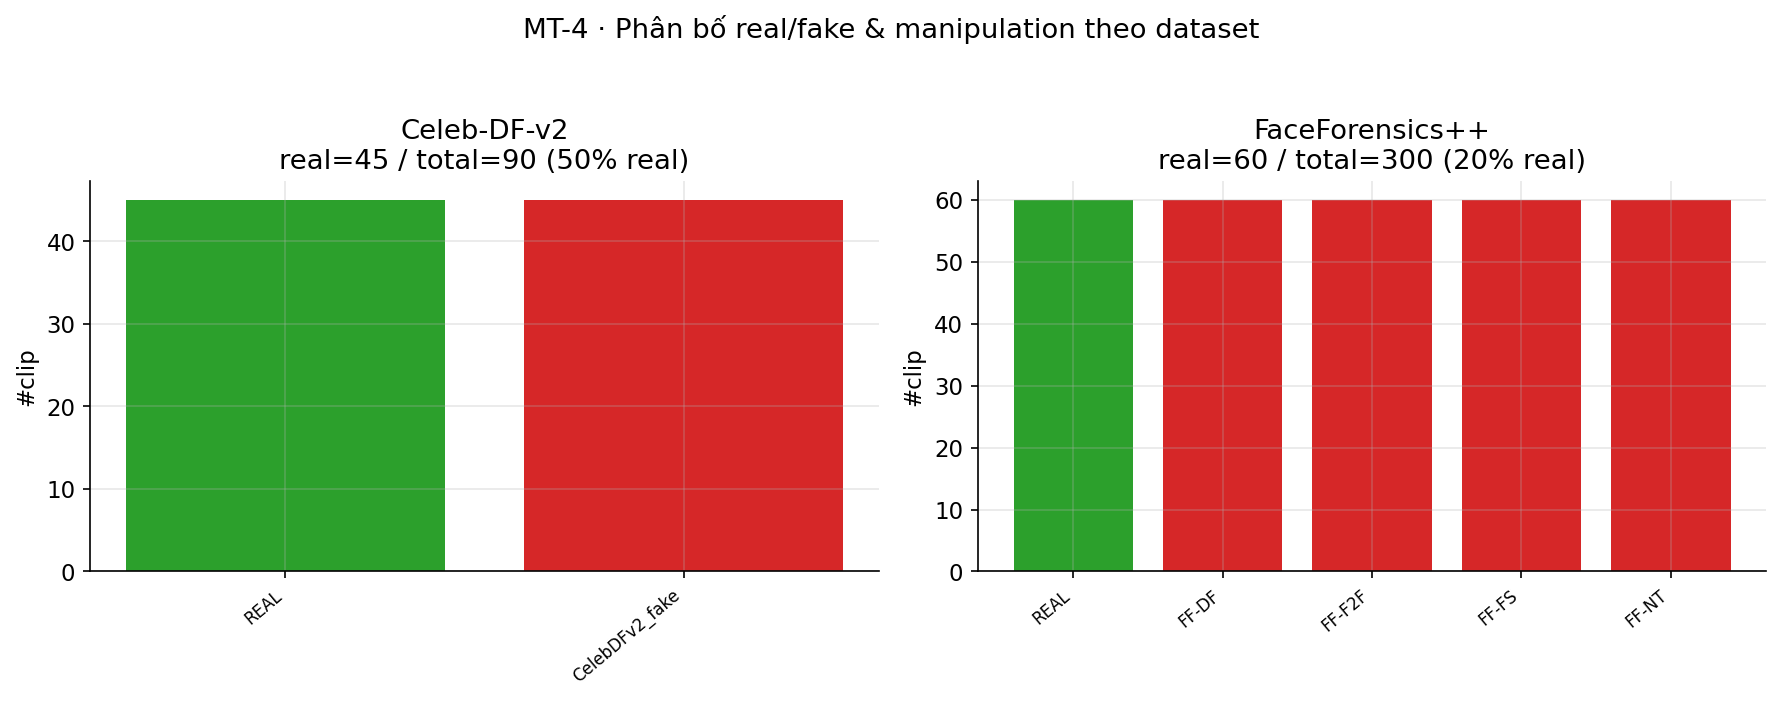
\includegraphics[width=0.92\linewidth]{fig_3_1_distribution.png}
\caption{Real/fake distribution: FF++ (train) vs Celeb-DF-v2 (test).}\label{fig:dist}\end{figure}

\textbf{Pipeline sanity \& convergence.} B4 reaches 0.7497, matching the DeepfakeBench leaderboard
(0.7487), confirming a correct pipeline. Training curves (Figs.~\ref{fig:train}) are plotted directly
from real logs (no simulation).

\begin{figure}[t]\centering
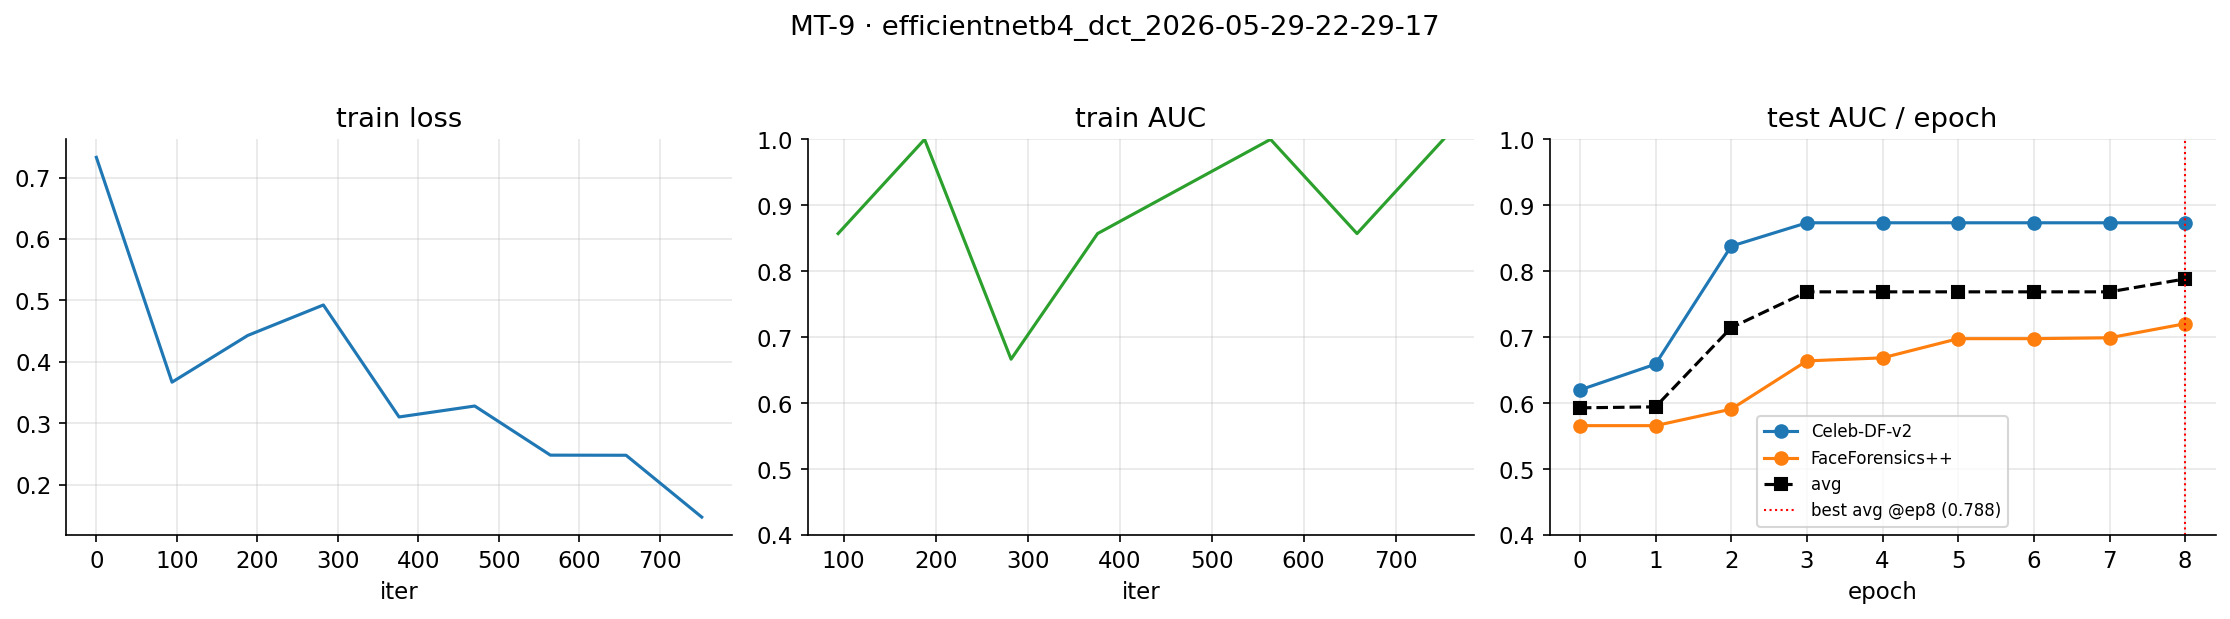
\includegraphics[width=0.99\linewidth]{fig_3_4_train_naive.png}
\caption{Training/validation curves of naive SFDCT (loss + per-epoch test-AUC), from real logs.}\label{fig:train}\end{figure}

\textbf{Main result (honest).} Table~\ref{tab:main} reports the ablation ladder. Adding the block-DCT
branch lifts AUC to 0.7572 ($\Delta{=}{+}0.0075$) \emph{without} regressing the baseline (floor holds).
A bootstrap confidence interval over the test scores gives $\Delta\text{AUC}\in[-0.004,+0.019]$
($p\approx0.18$): \textbf{the gain is within noise}; we therefore do not claim an AUC improvement, only
a non-regression with a safety guarantee. Row1 (0.7333) is \emph{below} B4, i.e.\ the ladder is not
monotonic --- shown openly, attributable to the missing gate/band-drop in that configuration.
ROC/PR curves are in Fig.~\ref{fig:roc}.

\begin{table}[t]\centering
\caption{Cross-dataset frame-AUC (train FF++ $\to$ test Celeb-DF-v2). Own single-seed runs.}\label{tab:main}
\begin{tabular}{lcc}\toprule
Model & CDFv2 frame-AUC & $\Delta$ vs B4 \\ \midrule
B4 (baseline) & 0.7497 & --- \\
naive SFDCT (B4-DCT) & \textbf{0.7572} & $+0.0075$ (in noise) \\
Row1 (S1+S2+S3) & 0.7333 & $-0.0164$ \\
Row2 (S4+S5+S3) & \multicolumn{2}{c}{\todo{training}} \\ \midrule
\multicolumn{3}{l}{\footnotesize Context (DeepfakeBench scale): SPSL 0.7650, SRM 0.7552, F3Net 0.7352.}\\
\bottomrule\end{tabular}\end{table}

\begin{figure}[t]\centering
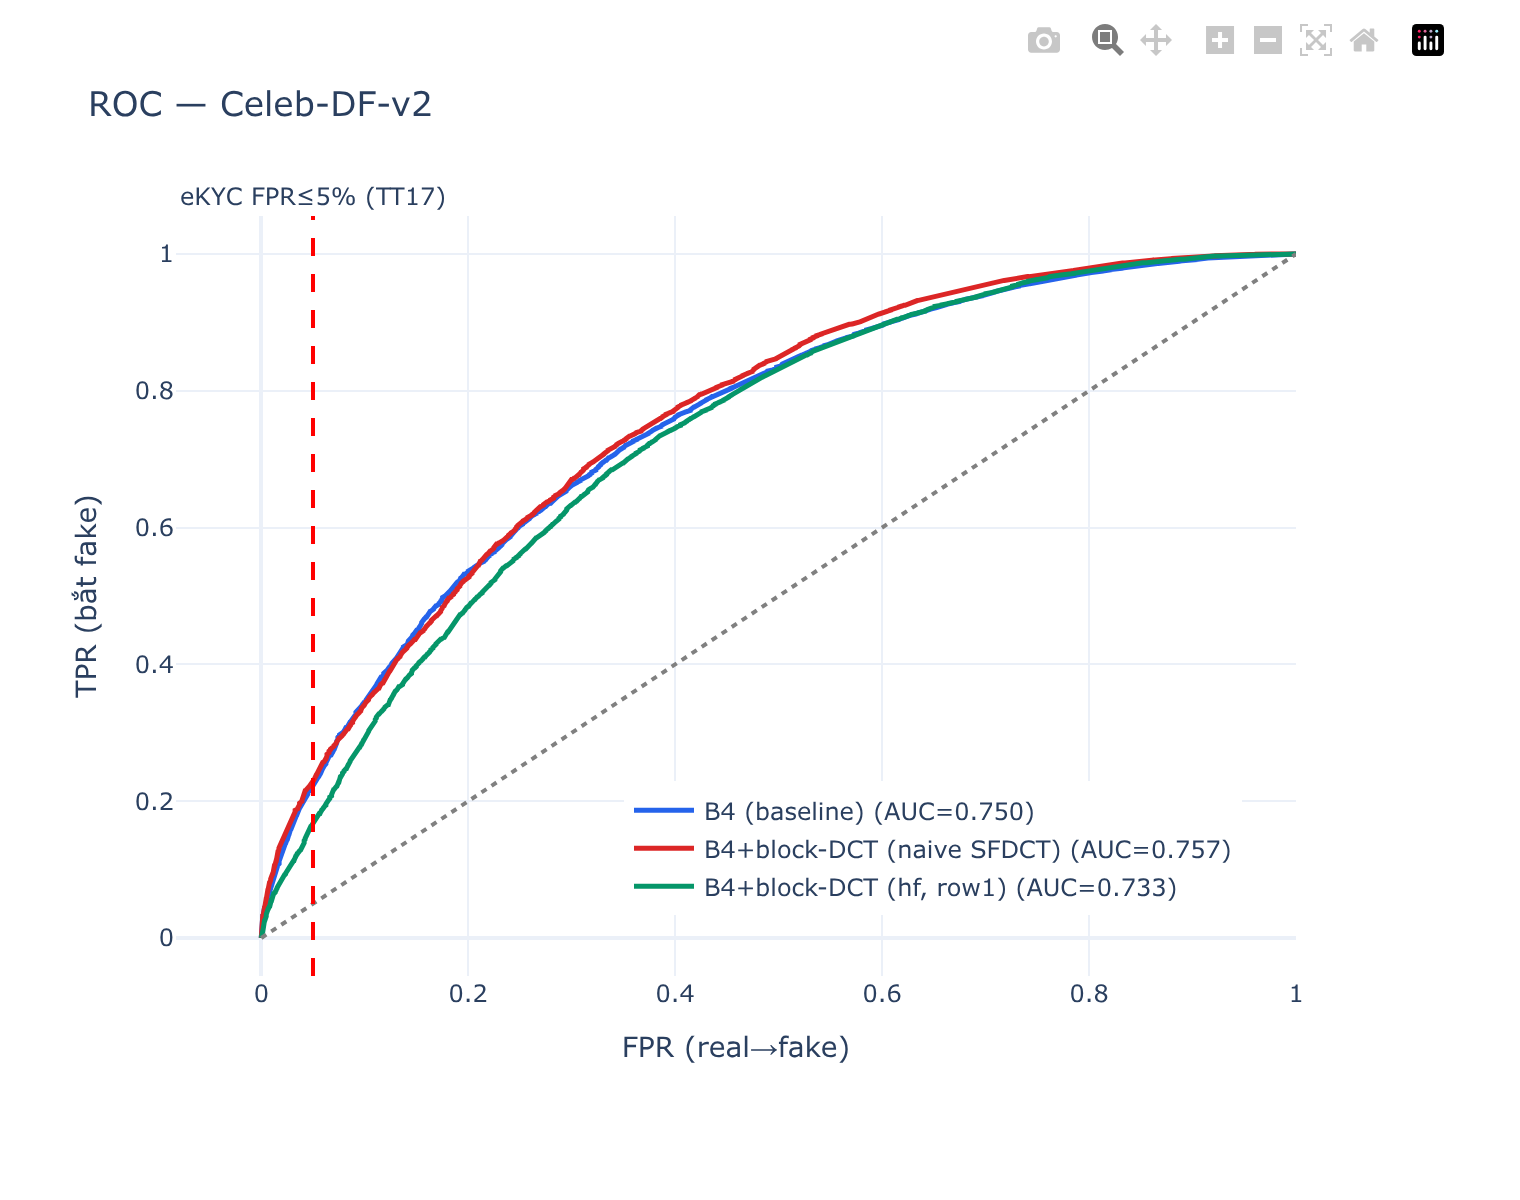
\includegraphics[width=0.85\linewidth]{fig_3_7_roc.png}
\caption{ROC on Celeb-DF-v2; red line marks the eKYC operating point $\text{FPR}\le5\%$.}\label{fig:roc}\end{figure}

\textbf{Per-knob ablation (S1--S5).} \todo{per-knob runs not yet available; only the cumulative
Row1/Row2 configurations exist.}

\subsection{eKYC operating-point evaluation}\label{sec:ekyc}
We calibrate $\tau$ at $\text{FPR}\le5\%$ (ISO/IEC~30107-3 convention; the circular itself sets no number).
For naive SFDCT, $\tau{=}0.9514$ gives test FPR $0.050$ and TPR $0.2298$. The confusion matrix
(Fig.~\ref{fig:cm}) is TN$=5339$, FP$=281$, FN$=8318$, TP$=2482$: the dominant error is
\emph{false negative} --- about 77\% of deepfakes pass at this real-user-friendly point. This is the
honest diagnostic: at $\text{AUC}\approx0.76$, neither operating end is acceptable alone (security-first
$\Rightarrow$ reject $\sim$69\% of genuine users; usability-first $\Rightarrow$ 77\% fakes pass). SFDCT
is suited as a \emph{first-stage screen} combined with liveness and video-level aggregation
(video-AUC 0.808 $>$ frame 0.757), not as a standalone gate.

\begin{figure}[t]\centering
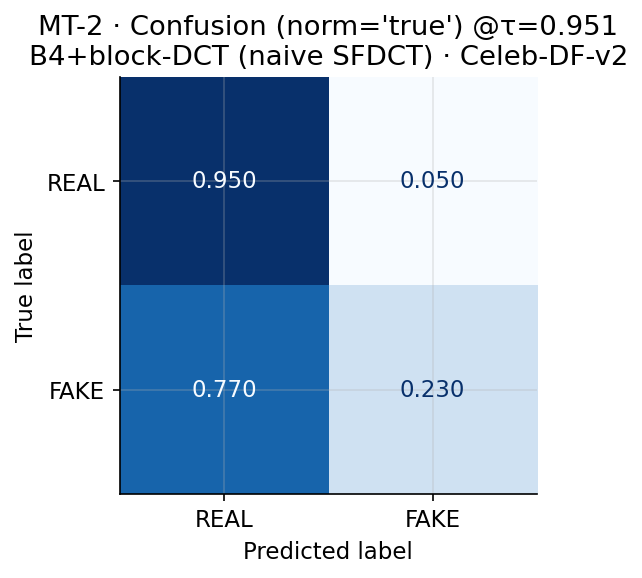
\includegraphics[width=0.7\linewidth]{fig_3_9_confusion.png}
\caption{Confusion (row-normalized) of naive SFDCT at $\tau$ for $\text{FPR}\le5\%$.}\label{fig:cm}\end{figure}

\subsection{Qualitative analysis}
Fig.~\ref{fig:freq} shows that real faces carry more mid/high-band DCT energy than fakes (deepfakes are
smoother), confirming a frequency signal --- though weak on c23 due to compression, which is precisely
why $\Delta$ is small. Grad-CAM (Fig.~\ref{fig:gcam}) shows SFDCT attends to face/blending regions, and
the learned gate $|\alpha|>0$ (Fig.~\ref{fig:gate}) confirms the frequency branch is engaged.

\begin{figure}[t]\centering
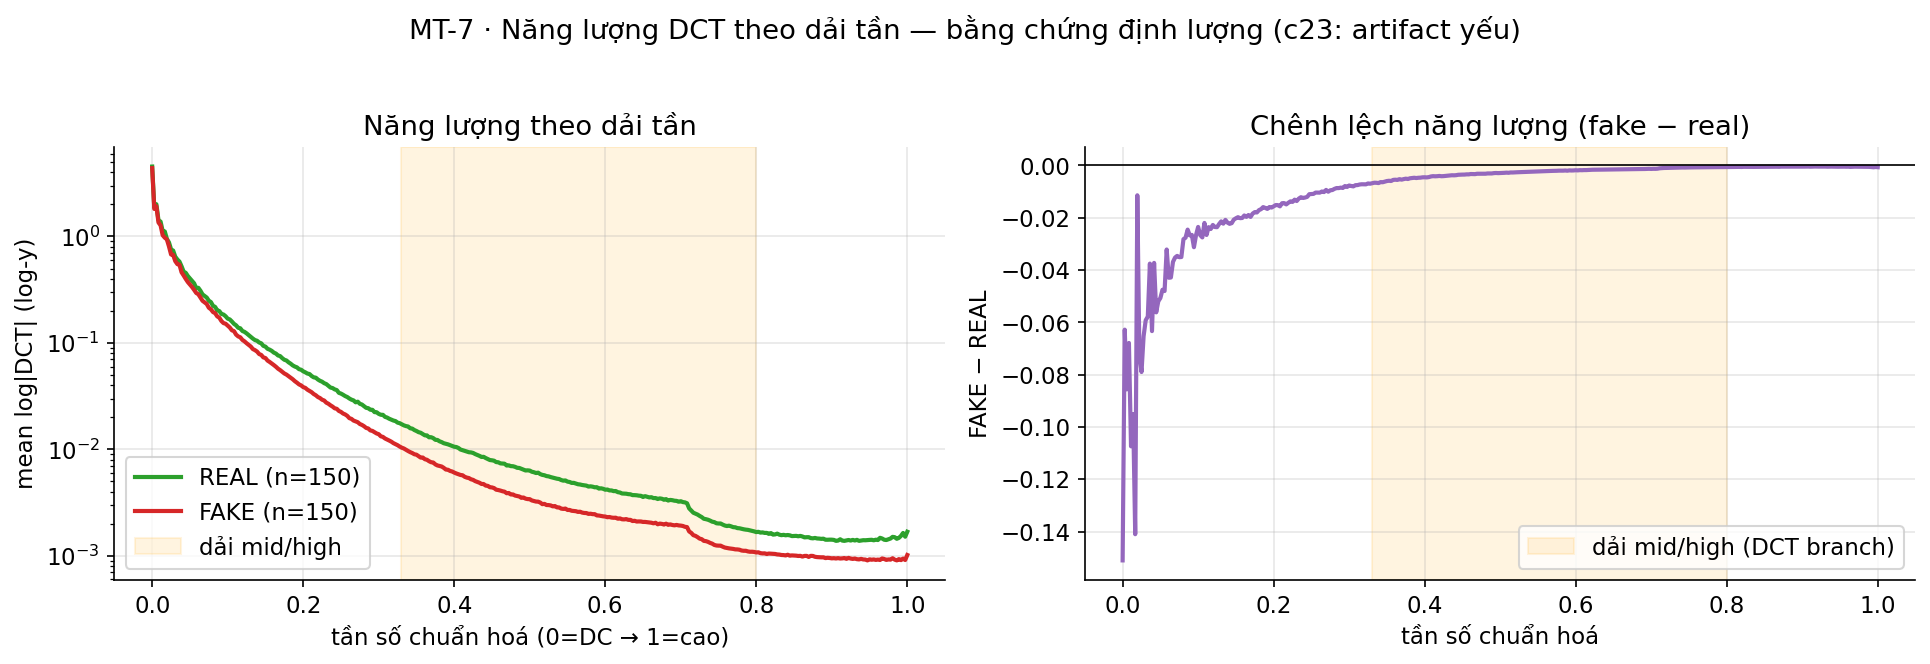
\includegraphics[width=0.99\linewidth]{fig_3_11_frequency.png}
\caption{Mean DCT energy by frequency band: real $>$ fake in mid/high bands.}\label{fig:freq}\end{figure}

\begin{figure}[t]\centering
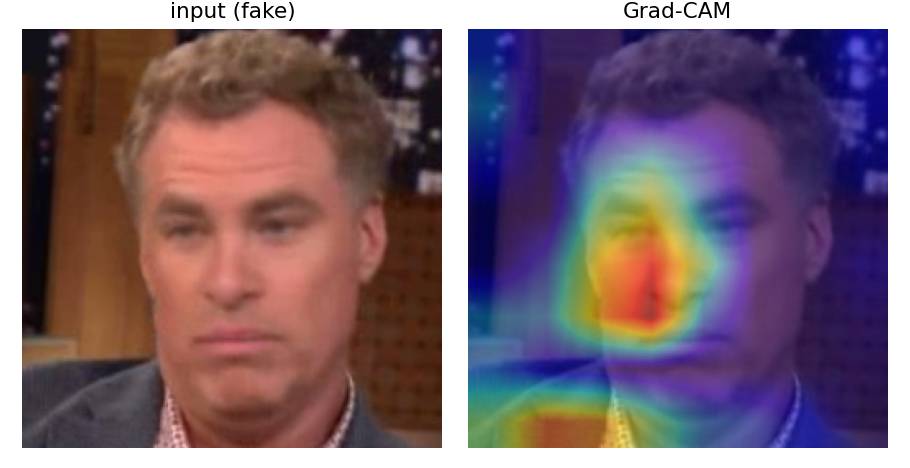
\includegraphics[width=0.8\linewidth]{fig_3_12_gradcam.png}
\caption{Grad-CAM of SFDCT on a Celeb-DF-v2 sample.}\label{fig:gcam}\end{figure}

\begin{figure}[t]\centering
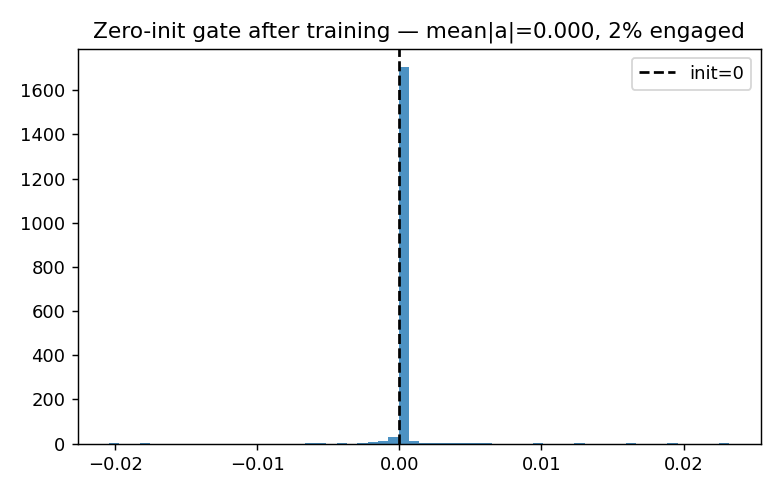
\includegraphics[width=0.75\linewidth]{fig_3_13_gate_alpha.png}
\caption{Learned gate $\alpha$ after training ($>0$): the DCT branch is actively used.}\label{fig:gate}\end{figure}

\section{Discussion and Limitations}\label{sec:limits}
We state limitations plainly. (1) $\Delta{=}{+}0.0075$ is within noise at frame level; a
\emph{video-level} bootstrap CI and multi-seed runs are required before any AUC claim
(\todo{video-level bootstrap}). (2) SFDCT does not surpass SPSL (0.7650). (3) Row1 $<$ B4 (non-monotonic).
(4) C1 is a new combination, not a new mechanism; the floor guarantee is a property of zero-init that
holds at initialization. (5) APCER/BPCER are PAD terms re-defined here for forgery. (6) The Vietnamese
test set (C3) is small and test-only and must ship with a datasheet, baselines, bootstrap CI, and an
ethics/consent statement (\todo{collect $\ge$30 videos, $\ge$2 generators}). (7) Frame-level results are
a lower-bound diagnostic; real eKYC decides at video/session level with liveness.

\section{Conclusion}
SFDCT contributes a floor-preserving spatial--frequency fusion, a regulation-aware eKYC operating-point
evaluation, and a localized Vietnamese-face test resource, built faithfully on DeepfakeBench. We make no
SOTA claim: the AUC gain is within noise, and the value lies in the safety guarantee, the honest
eKYC-anchored diagnostic, and the localized resource. Future work: video-level bootstrap, per-knob
ablation, and the SBI/FSBI route toward the modern generalization tier.

\bibliographystyle{IEEEtran}
\bibliography{references}
\end{document}
